%杨舒云的实验报告编辑界面,使用了Huanyu Shi,2019级的模板,杨舒云在此拜谢ORZ!

%!TEX program = xelatex
\documentclass[dvipsnames, svgnames,a4paper,11pt]{article}
% ----------------------------------------------------- 
%	加边框的命令
%	参考:https://tex.stackexchange.com/questions/531559/how-to-add-the-page-border-for-first-two-pages-in-latex
\usepackage{tikz}
\usetikzlibrary{calc}
\usepackage{eso-pic}
\AddToShipoutPictureBG{%
\begin{tikzpicture}[overlay,remember picture]
\draw[line width=0.6pt] % 边框粗细
    ($ (current page.north west) + (0.6cm,-0.6cm) $)
    rectangle
    ($ (current page.south east) + (-0.6cm,0.6cm) $); % 边框位置
\end{tikzpicture}}


\usepackage{xcolor}
\definecolor{c1}{HTML}{086173} % 目录颜色 原版为2752C9 紫灰色535AAA 蓝紫色0B0DB7 深蓝色070F94 湖绿色219394 松石灰绿086173
\definecolor{c2}{HTML}{E20129} % 引用颜色 原版\definecolor{c2}{RGB}{190,20,83} 橙色F24729

\usepackage{ctex}
\usepackage[top=28mm,bottom=28mm,left=15mm,right=15mm]{geometry}
\usepackage{hyperref} 
\hypersetup{
	colorlinks,
	linktoc = section, % 超链接位置,选项有section, page, all
	linkcolor = c1, % linkcolor 目录颜色
	citecolor = c1  % citecolor 引用颜色
}
\usepackage{amsmath,enumerate,multirow,float}
\usepackage{tabularx}
\usepackage{tabu}
\usepackage{subfig}
\usepackage{fancyhdr}
\usepackage{graphicx}
\usepackage{wrapfig}  
\usepackage{physics}
\usepackage{appendix}
\usepackage{amsfonts}

%
\usepackage{tcolorbox}
\tcbuselibrary{skins,breakable}
\newtcolorbox{tbox}[2][]{
    colframe=black!70!,
    breakable,
    enhanced,
	boxrule =0.5pt,
    title = {#2},
    fonttitle = \large\kaishu\bfseries,
	drop fuzzy shadow,
    #1
}
\newtcolorbox[auto counter,number within=section]{question}[1][]{
  top=2pt,bottom=2pt,arc=1mm,
  boxrule=0.5pt,
%   frame hidden,
  breakable,
  enhanced, %跨页后不会显示下边框
  coltitle=c1!80!gray,
  colframe=c1,
  colback=c1!3!white,
  drop fuzzy shadow,
  title={思考题~\thetcbcounter:\quad},
  fonttitle=\bfseries,
  attach title to upper,
  #1
}

% ---------------------------------------------------------------------
%	利用cleveref改变引用格式,\cref是引用命令
\usepackage{cleveref}
\crefformat{figure}{#2{\textcolor{c2}{Figure #1}}#3} % 图片的引用格式
\crefformat{equation}{#2{(\textcolor{c2}{#1})}#3} % 公式的引用格式
\crefformat{table}{#2{\textcolor{c2}{Table #1}}#3} % 表格的引用格式


% ---------------------------------------------------------------------
%	页眉页脚设置
\fancypagestyle{plain}{\pagestyle{fancy}}
\pagestyle{fancy}
\lhead{\kaishu 中山大学物理与天文学院电子技术实验\uppercase\expandafter{\romannumeral1}} % 左边页眉,学院 + 课程
\rhead{\kaishu 实验报告By戴鹏辉、杨舒云} % 右边页眉,实验报告标题
\cfoot{\thepage} % 页脚,中间添加页码


% ---------------------------------------------------------------------
%	对目录、章节标题的设置
\renewcommand{\contentsname}{\centerline{\huge 目录}}
\usepackage{titlesec}
\usepackage{titletoc}
% \titleformat{章节}[形状]{格式}{标题序号}{序号与标题间距}{标题前命令}[标题后命令]
\titleformat{\section}{\centering\LARGE\songti}{}{1em}{}

% ---------------------------------------------------------------------
%   listing代码环境设置
\usepackage{listings}
\lstloadlanguages{python}
\lstdefinestyle{pythonstyle}{
backgroundcolor=\color{gray!5},
language=python,
frameround=tftt,
frame=shadowbox, 
keepspaces=true,
breaklines,
columns=spaceflexible,                   
basicstyle=\ttfamily\small, % 基本文本设置,字体为teletype,大小为scriptsize
keywordstyle=[1]\color{c1}\bfseries, 
keywordstyle=[2]\color{Red!70!black},   
stringstyle=\color{Purple},       
showstringspaces=false,
commentstyle=\ttfamily\scriptsize\color{green!40!black},%注释文本设置,字体为sf,大小为smaller
tabsize=2,
morekeywords={as},
morekeywords=[2]{np, plt, sp},
numbers=left, % 代码行数
numberstyle=\it\tiny\color{gray}, % 代码行数的数字字体设置
stepnumber=1,
rulesepcolor=\color{gray!30!white}
}




% ---------------------------------------------------------------------
%	其他设置
\def\degree{${}^{\circ}$} % 角度
\graphicspath{{./images/}} % 插入图片的相对路径
\allowdisplaybreaks[4]  %允许公式跨页 
\usepackage{lipsum}
\usepackage{adjustbox}
%\usepackage{mathrsfs} % 字体
\captionsetup[figure]{name=Figure} % 图片形式
\captionsetup[table]{name=Table} % 表格形式

\begin{document}
	
	
	
	% 实验报告封面	
	
	% 顶栏
	\begin{table}
		\renewcommand\arraystretch{1.7}
		\begin{tabularx}{\textwidth}{
				|X|X|X|X
				|X|X|X|X|}
			\hline
			\multicolumn{2}{|c|}{预习报告}&\multicolumn{2}{|c|}{实验记录}&\multicolumn{2}{|c|}{分析讨论}&\multicolumn{2}{|c|}{总成绩}\\
			\hline
			\LARGE25 & & \LARGE25 & & \LARGE30 & & \LARGE80 & \\
			\hline
		\end{tabularx}
	\end{table}
	% ---
	
	% 信息栏
	\begin{table}
		\renewcommand\arraystretch{1.7}
		\begin{tabularx}{\textwidth}{|X|X|X|X|}
			\hline
			年级、专业: & 2022级 物理学 &组号: & 2\\
			\hline
			姓名: & 戴鹏辉、杨舒云  & 学号: & 22344016、223444020\\
			\hline
			实验时间: & 2024// & 教师签名: & \\
			\hline
		\end{tabularx}
	\end{table}
	% ---
	
	% 大标题
	\begin{center}
		\LARGE ETX \quad 实验名称×××
	\end{center}
	% ---
	
	% 注意事项
	
	% 基本
	\textbf{【实验报告注意事项】}
	\begin{enumerate}
		\item 实验报告由三部分组成:
		\begin{enumerate}
			\item 预习报告:课前认真研读实验讲义,弄清实验原理;实验所需的仪器设备、用具及其使用、完成课前预习思考题;了解实验需要测量的物理量,并根据要求提前准备实验记录表格(可以参考实验报告模板,可以打印)。\textcolor{red}{\textbf{(20分)}}
			\item 实验记录:认真、客观记录实验条件、实验过程中的现象以及数据。实验记录请用珠笔或者钢笔书写并签名(\textcolor{red}{\textbf{用铅笔记录的被认为无效}})。\textcolor{red}{\textbf{保持原始记录,包括写错删除部分,如因误记需要修改记录,必须按规范修改。}}(不得输入电脑打印,但可扫描手记后打印扫描件);离开前请实验教师检查记录并签名。\textcolor{red}{\textbf{(30分)}}
			\item 数据处理及分析讨论:处理实验原始数据(学习仪器使用类型的实验除外),对数据的可靠性和合理性进行分析;按规范呈现数据和结果(图、表),包括数据、图表按顺序编号及其引用;分析物理现象(含回答实验思考题,写出问题思考过程,必要时按规范引用数据);最后得出结论。\textcolor{red}{\textbf{(30分)}}
		\end{enumerate}
		\textbf{实验报告就是将预习报告、实验记录、和数据处理与分析合起来,加上本页封面。\textcolor{red}{(80分)}}
		\item 每次完成实验后的一周内交\textbf{实验报告}(特殊情况不能超过两周)。
		\item \textbf{其它注意事项}:
		\begin{enumerate}
			\item 请认真查看并理解实验讲义第一章内容;
			\item 注意实验器材的合理使用;
			\item 使用结束使用各种仪器之后需要将其放回原位。
		\end{enumerate}
	\end{enumerate}
	
	% 安全
	\textbf{【实验安全注意事项】}	
	\begin{enumerate}
		\item 
	\end{enumerate}
	
	% ---
	
	% 特别鸣谢
	\textbf{【特别鸣谢及模板说明】}	
	
	感谢2019级学长石寰宇为本实验报告提供\LaTeX 模板。\textcolor{red}{\textbf{由于原实验报告模板缺少实验编号,为方便在电脑上整理,故添加自命名编号}}
	% ---
	
	
	
	% 目录
	\clearpage
	\tableofcontents
	\clearpage
	% ---
	
	
	
	% 预习报告	
	
	% 小标题
	\setcounter{section}{0}
	\section{ETX 实验名称××× \quad\heiti 预习报告}
	% ---
	
	% 实验目的
	\subsection{实验目的}
	\begin{enumerate}
		\item 
	\end{enumerate}
	% ---
	
	% 仪器用具
	\subsection{仪器用具}
	\begin{table}[htbp]
		\centering
		\renewcommand\arraystretch{1.6}
		% \setlength{\tabcolsep}{10mm}
		\begin{tabular}{p{0.05\textwidth}|p{0.20\textwidth}|p{0.05\textwidth}|p{0.5\textwidth}}
			\hline
			编号& 仪器用具名称 & 数量 &  主要参数(型号,测量范围,测量精度等) \\
			\hline
			1&  & 1 &  \\
			\hline
		\end{tabular}
	\end{table}
	% ---
	
	% 原理概述
	\subsection{原理概述}
	\begin{enumerate}
		\item 
	\end{enumerate}
	% ---
	
	
	
	% 实验前思考题
	\subsection{实验预习题}
	
	% 思考题1
	\begin{question}
		
	\end{question}
	
	% 思考题2
	\begin{question}
		
	\end{question}
	
	% 思考题3
	\begin{question}
		
	\end{question}
	
	% ---
	
	
	
	% 实验记录	
	\clearpage
	
	% 顶栏
	\begin{table}
		\renewcommand\arraystretch{1.7}
		\centering
		\begin{tabularx}{\textwidth}{|X|X|X|X|}
			\hline
			专业: & 物理学 & 年级: & 2022级 \\
			\hline
			姓名: & 戴鹏辉、杨舒云 & 学号: & 22344016、22344020\\
			\hline
			室温: &  & 实验地点: & A522 \\
			\hline
			学生签名:& 见\textbf{附件}部分 & 评分: &\\
			\hline
			实验时间:& 2024// & 教师签名:&\\
			\hline
		\end{tabularx}
	\end{table}
	% ---
	
	% 小标题
	\section{ETX 实验名称×××  \quad\heiti 实验记录}
	% ---
	
	% 实验过程记录
	\subsection{实验内容、步骤与结果}
	
	%
	\subsubsection{操作步骤记录}
	\begin{enumerate}
		\item 
	\end{enumerate}	
	
	%
	\subsubsection{}
	\begin{enumerate}
		\item \begin{table}[h]
			\centering
			\caption{表格示例}
			\label{tab:tab1}
			\begin{tabular}{|c|c|c|c|c|c|}
				\hline
				组1/序号i & 1 & 2 & 3 & 4 & 5 \\
				$v_{1i}(m/s)$ & 1.26 & 1.08 & 1.00 & 0.75 & 0.38 \\
				$f_{1i}(Hz)$ & 40073 & 40127 & 40105 & 40088 & 40066 \\
				\hline
				组2/序号i & 1 & 2 & 3 & 4 & 5 \\
				$v_{2i}(m/s)$ & 1.21 & 1.06 & 0.99 & 0.52 & 0.57 \\
				$f_{2i}(Hz)$ & 40143 & 40125 & 40084 & 40080 & 40067 \\
				\hline
				组3/序号i & 1 & 2 & 3 & 4 & 5 \\
				$v_{3i}(m/s)$ & 1.15 & 0.98 & 0.78 & 0.59 & 0.36 \\
				$f_{3i}(Hz)$ & 40135 & 40115 & 40092 & 40070 & 40044 \\
				\hline
			\end{tabular}
		\end{table}		
	\end{enumerate}
	
	% ---
	
	% 原始数据
	\clearpage
	\subsection{原始数据记录}
	实验记录本上的原始数据见%\cref{}(签字)。
	
	实验台桌面整理见%\textbf{附件}部分(\cref{})。
	
	其它原始数据见%\cref{}。
	% ---
	
	% 问题记录
	\subsection{实验过程遇到问题及解决办法}
	\begin{enumerate}
		\item 
	\end{enumerate}
	% ---
	
	
	
	% 分析与讨论	
	\clearpage
	
	% 顶栏
	\begin{table}
		\renewcommand\arraystretch{1.7}
		\begin{tabularx}{\textwidth}{|X|X|X|X|}
			\hline
			专业:& 物理学 &年级:& 2022级\\
			\hline
			姓名: & 戴鹏辉、杨舒云 & 学号:& 22344016、22344020\\
			\hline
			日期:& 2024// & 评分: &\\
			\hline
		\end{tabularx}
	\end{table}
	% ---
	
	% 小标题
	\section{ETX 实验名称××× \quad\heiti 分析与讨论}
	% ---
	
	% 数据处理
	\subsection{实验数据分析}
	
	%
	\subsubsection{}
	\begin{enumerate}
		\item 
	\end{enumerate}
	
	%
	\subsubsection{}
	\begin{enumerate}
		\item 
	\end{enumerate}
	
	%
	\subsubsection{}
	
	% ---
	
	% 实验后思考题
	\subsection{实验后思考题}
	
	%思考题1
	\begin{question}
		
	\end{question}
	
	% 思考题2
	\begin{question}
		
	\end{question}
	
	% 思考题3
	\begin{question}
		
	\end{question}
	
	% ---
	
	
	% 结语部分
	\clearpage
	
	% 小标题
	\section{ETX 实验名称××× \quad\heiti 结语}
	% ---
	
	% 总结、杂谈与致谢
	\subsection{实验心得和体会、意见建议等}
	\begin{enumerate}
		\item 
	\end{enumerate}
	% ---
	
	% 参考文献
	\subsection{参考文献}
	[1] 维基百科 https://zh.wikipedia.org
	
	[2] 沈韩.基础物理实验.——北京:科学出版社,2015.2 ISBN:978-7-03-043311-4
	
	% ---
	
	% 附件
	\subsection{附件及实验相关的软硬件资料等}
	试验台桌面整理如%\cref{}所示。
	
	实验报告个人签名如\cref{fig:name}。
	
	\begin{figure}[htbp]
		\centering
		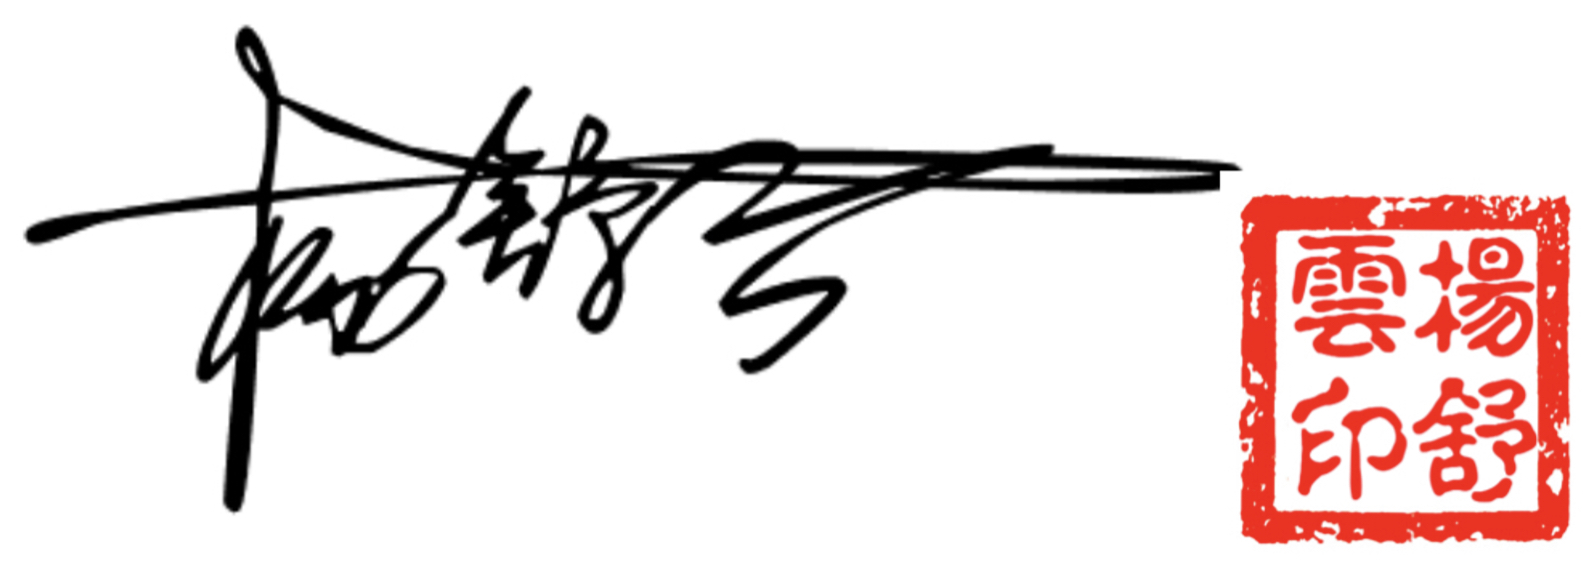
\includegraphics[width=0.7\textwidth]{name.png}
		\caption{个人签名}
		\label{fig:name}
	\end{figure}
	
	% ---
	
	相关代码已上传至Github。
	
	
	
\end{document}